% !TeX TS-program = xelatex

\documentclass{beamer}

\usepackage{tabularx}
\usepackage{xltxtra}
\usepackage{fontspec}
\usepackage{polyglossia}
\usepackage{makecell}
\usepackage{listings}

\usepackage{circuitikz}
\usepackage{tikz}
\usetikzlibrary{arrows.meta,calc,decorations.markings,math,arrows.meta,shapes,arrows,decorations.pathreplacing}
\usetikzlibrary{positioning}

\tikzset{block/.style = {draw, fill=white, rectangle,
		minimum height=3em, minimum width=2cm},
	input/.style = {coordinate},
	output/.style = {coordinate},
	pinstyle/.style = {pin edge={to-,t,black}},
	radiation/.style={decorate,decoration={expanding waves,angle=12,segment length=4pt}}
}

\setbeamertemplate{endpage}{%
	\begin{frame}
		\begin{center}
			\Huge Demo
		\end{center}
	\end{frame}
}


\setdefaultlanguage{german}

\usetheme[blue]{Verona}
\usefonttheme{default}
\usefonttheme{professionalfonts}

\usefonttheme[stillsansseriftext]{serif}

\defaultfontfeatures{Ligatures=TeX,Scale=MatchLowercase}
\setsansfont{Segoe UI Light}
\setmainfont{Segoe UI}
\setmonofont{Impact}


\title{Message Queuing Telemetry Transport}
\subtitle{Implementierung einer IoT-Anwendung auf Basis von MQTT}
\author{Maximilian Gaul, Lukas Dorner}
\date{01.07.2019}

%\mode<presentation>

\begin{document}
	
\begin{frame}
	\titlepage
\end{frame}

\begin{frame}

\frametitle{Paper}
\framesubtitle{Internet of Things: A Survey on Enabling Technologies, Protocols, and Applications}
\begin{itemize}
	\item Idee, IoT-Projekte in 5 Layer aufzuteilen
	\begin{itemize}
		\item \textbf{Objects Layer}: Physikalischer Sensoren und Aktuatoren, die verschiedene Funktionen übernehmen
		\item \textbf{Object Abstraction Layer}: Transport der Daten zum nächsten Layer, z.B. über WiFi, Bluetooth
		\item \textbf{Service Management Layer}: Verarbeitet und abstrahiert empfangene Daten bzw. die Hardwareplattform
		\item \textbf{Application Layer}: Stellt den Anwendern die Daten zur Verfügung, die sie benötigen (z.B. Temperaturdaten)
		\item \textbf{Business Layer}: Verwaltung der gesamten IoT-Applikation, Verwendung der Daten für z.B. \textit{Big Data}
	\end{itemize}
\end{itemize}

\end{frame}

\begin{frame}

\frametitle{Projektidee im IoT-Bereich}
\framesubtitle{WiFi?, Bluetooth?, MQTT?, Temperatursensor?}
\begin{itemize}
	\item Viele verschiedene Hardware- und Protokollkombinationen denkbar \begin{center}
		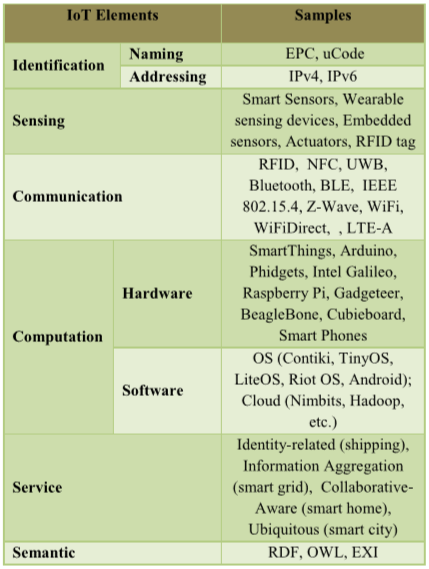
\includegraphics[scale=0.45]{images/iot_element.png}
	\end{center}
\end{itemize}

\end{frame}

\begin{frame}

\frametitle{Projektidee im IoT-Bereich}
\framesubtitle{WiFi, MQTT, Temperatursensor}
\begin{center}
	\begin{tikzpicture}
	\node (A) [anchor=south west,inner sep=0] at (0,0) {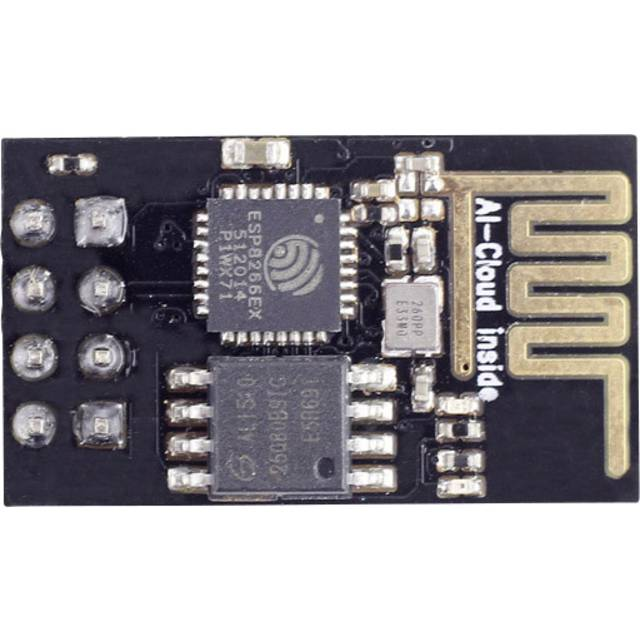
\includegraphics[scale=0.1]{images/esp8266.jpg}};
	\node (B) [right = of A] at (0,0) {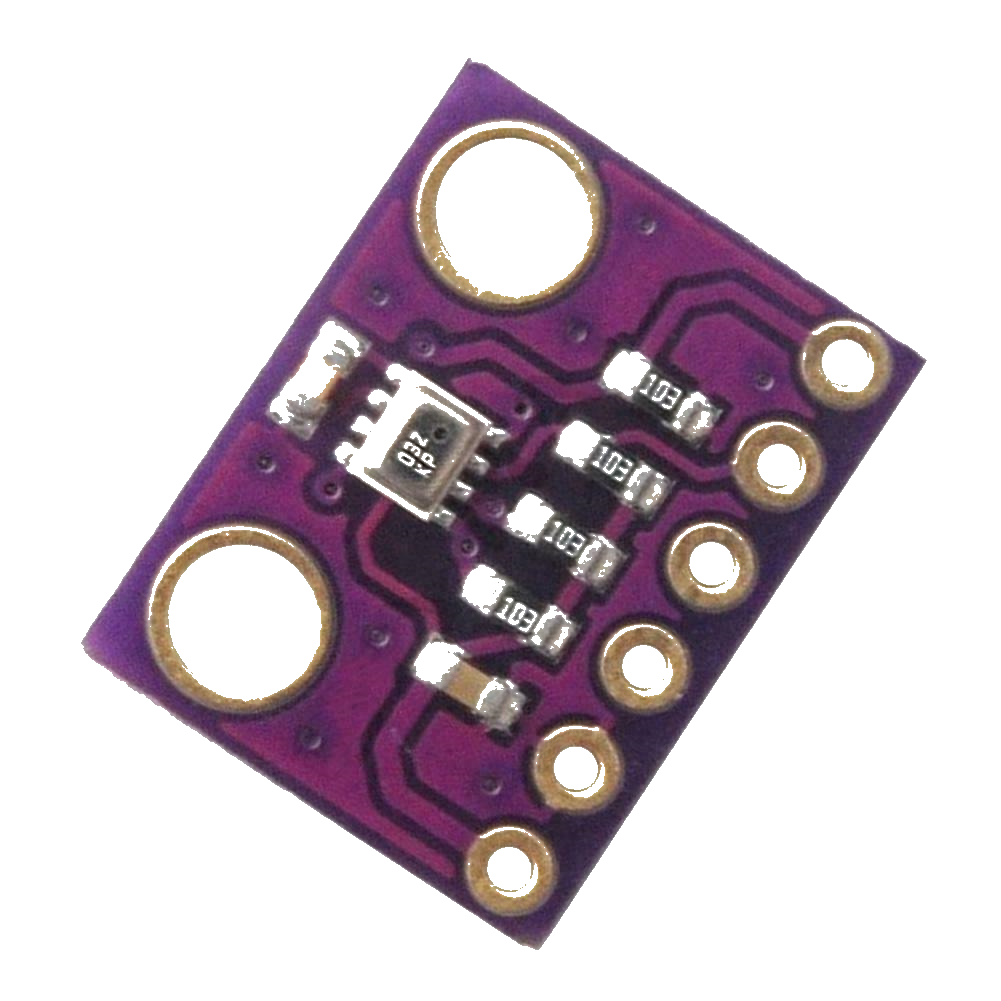
\includegraphics[scale=0.037]{images/bmp280.png}};
	\node (C) [below = of B] {ESP8266 + BMP280};
	
	\node (D) [right = 8cm of B] at (0,0) {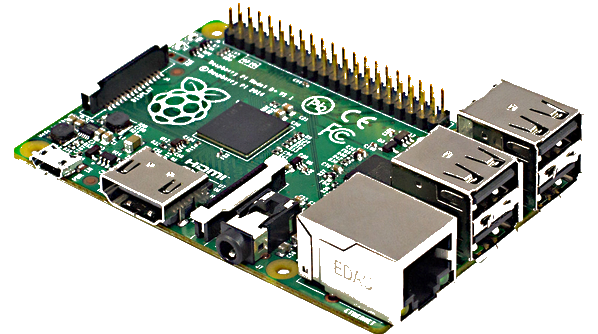
\includegraphics[scale=0.175]{images/raspi.png}};
	\node (E) [below = of D] {Raspberry Pi + Mosquitto};
	
	\draw[radiation] ([shift={(1cm,2cm)}]A)-- node [above=7mm] {MQTT} ([shift={(-1cm,2cm)}]D);
\end{tikzpicture}
\end{center}

\end{frame}

\begin{frame}

\frametitle{Projektidee im IoT-Bereich}
\framesubtitle{WiFi, MQTT, Temperatursensor}
\begin{tabularx}{\textwidth}{XXX}
	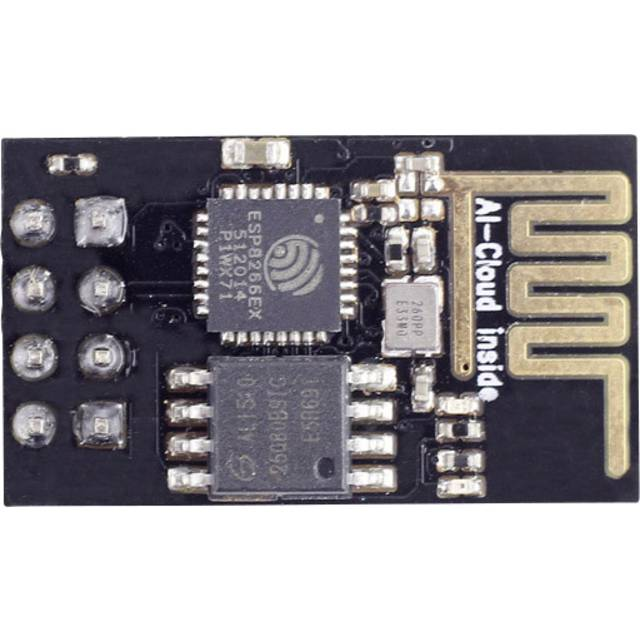
\includegraphics[scale=0.1]{images/esp8266.jpg} & 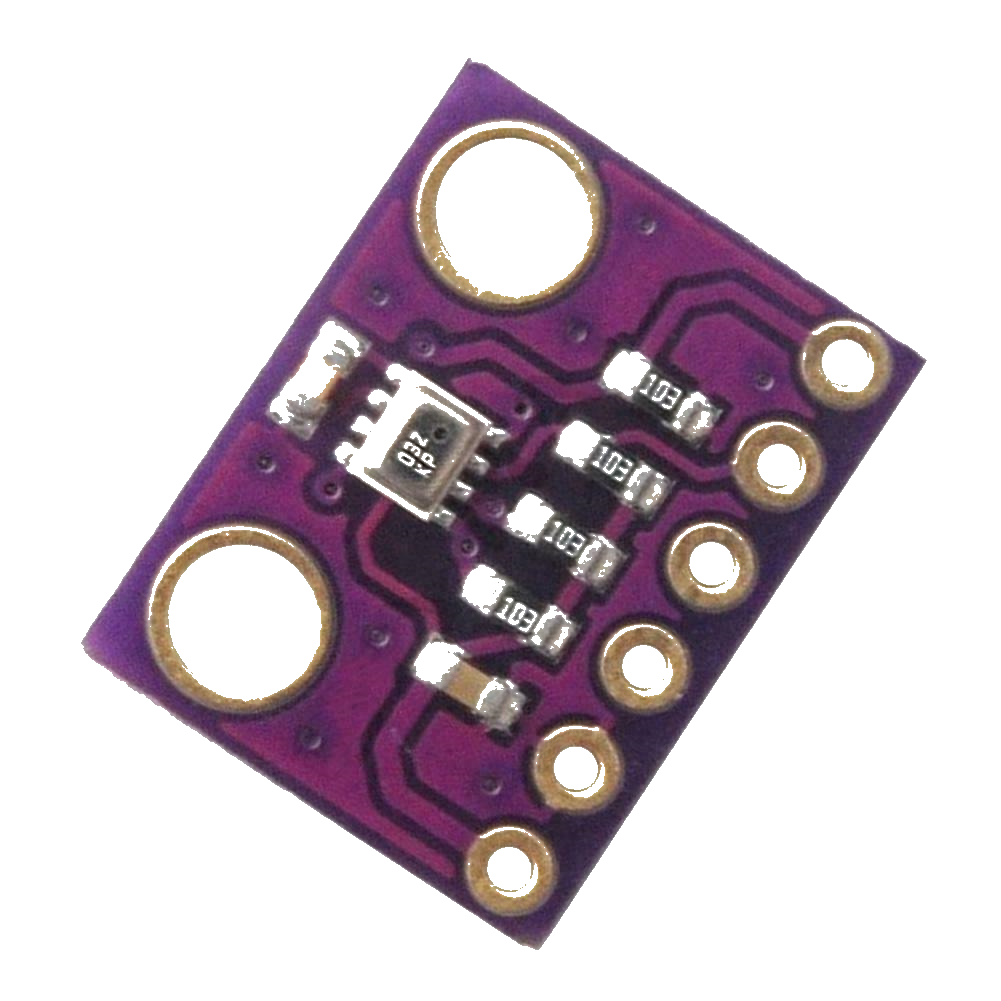
\includegraphics[scale=0.05]{images/bmp280.png} & 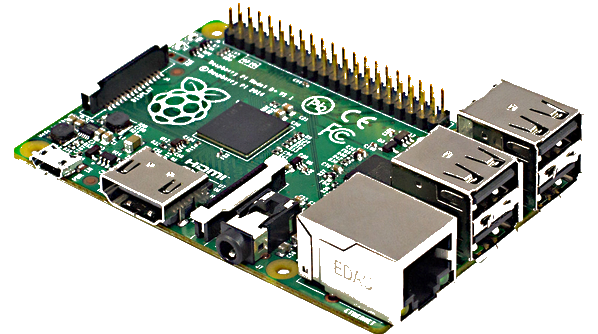
\includegraphics[scale=0.15]{images/raspi.png} \\
	\begin{itemize}
		\item 32-Bit \textit{RISC}- Controller, unterstützt 802.11 b/g/n mit bis zu 72.2Mbps
		\item 96 KByte RAM, 4 MB Flash
		\item Soft-I2C Anbindung an BMP280
	\end{itemize} & \begin{itemize}
		\item Temperatur- und Drucksensor
		\item 20-Bit Auflösung
		\item I2C-Interface
	\end{itemize} & \begin{itemize}
		\item Raspbian OS
		\item Mosquitto MQTT Broker \& Subscriber
	\end{itemize}
\end{tabularx}

\end{frame}

\begin{frame}

\frametitle{Projektumsetzung}
\framesubtitle{Implementierung von MQTT-CONNECT \& MQTT-PUBLISH auf ESP8266}
ESP8266 verbindet sich mit MQTT-CONNECT zum Mosquitto-Broker auf Raspi
\begin{itemize}
	\item Protokol-Name und Version
	\item Art der Verbindung
	\item \textit{Keep-Alive}
	\item Client ID
	\item \raisebox{-.5\height}{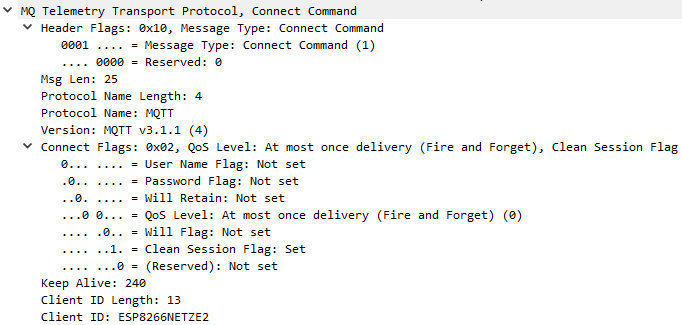
\includegraphics[scale=0.55]{images/wireshark_mqtt_connect.png}}
	
\end{itemize}

\end{frame}

\begin{frame}

\frametitle{Projektumsetzung}
\framesubtitle{Implementierung von MQTT-CONNECT \& MQTT-PUBLISH auf ESP8266}
ESP8266 sendet Temperaturdaten mit MQTT-PUBLISH an Mosquitto-Broker auf Raspi
\begin{itemize}
	\item \textit{QoS}-Flags
	\item Topic
	\item Payload (Temperaturdaten)
	\item \raisebox{-.5\height}{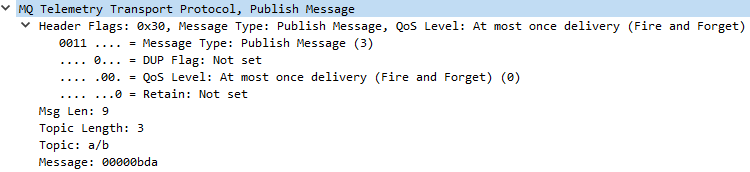
\includegraphics[scale=0.55]{images/wireshark_mqtt_publish.png}}
	
\end{itemize}

\end{frame}

\begin{frame}

\frametitle{Projektumsetzung}
\framesubtitle{Raspi \& Mosquitto}

\end{frame}


\begin{frame}

\frametitle{Projektumsetzung}
\framesubtitle{Raspi \& Mosquitto}

\end{frame}


\usebeamertemplate{endpage}


\end{document}